\documentclass[11pt]{article}
\title{Meccano pentagons gallery}
\author{https://github.com/heptagons/meccano/penta/gallery}
\date{}

\usepackage{../../meccano}
\begin{document}

\maketitle
\begin{abstract}
We show constructions of meccano rigid regular pentagons from side $12$ to $3$. We restrict all internal strips, we call diagonals, to remain inside the pentagon's perimeter and that don't overlap.
Several programs found the solutions and we show some alternatives and prove the claimed values are exact.
\end{abstract}

\section{Pentagons of size 12}

A program found that side 12 is the smallest pentagon that can be made rigid with a rhoumbus and two strips as diagonals so need only 4 strips as diagonals. We show two cases.

\begin{figure}[h]
 \centering
 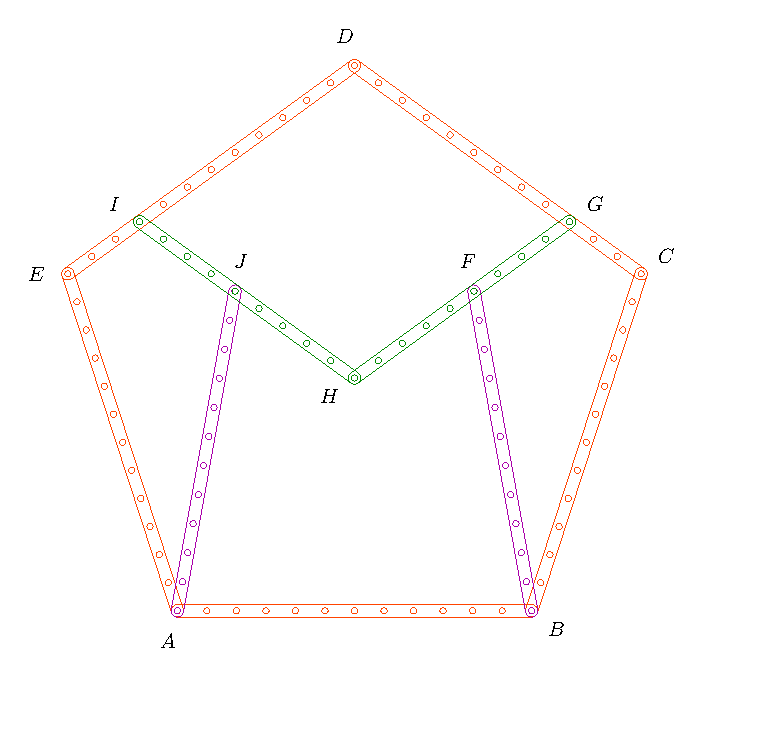
\includegraphics[scale=1]{12/penta12a}
 \caption{Pentagon size 12 (case a).}
 \label{fig:penta12a}
\end{figure}

Figure \ref{fig:penta12a} show a regular pentagon $A,B,C,D,E$ of side 12 with a rhombus $D,I,H,G$ of side $9$. We prove strips $AJ,BF$ are correct. First we calculate the abscissas going through vertices $A,E,I,J$ substracting when we move to the left and adding when we move to the right:
\begin{align}
AJ_x &= AE_x + EI_x + IJ_x\\
 &= -\overline{AE}\cos\left(\frac{2\pi}5\right)
 + \overline{EI}\cos\left(\frac{\pi}5\right) 
 + \overline{IJ}\cos\left(\frac{\pi}5\right)\nonumber\\
 &= -12\left(\frac{\sqrt5 - 1}4\right)
  +3\left(\frac{1+\sqrt5}4\right)
  +4\left(\frac{1+\sqrt5}4\right) = \frac{19-5\sqrt5}4
\end{align}

Then we calculate the ordinates going to the same order of vertices adding when we go up and substracting when we go down:
\begin{align}
AJ_y &= -AE_y + EI_y + IJ_y\\
 &= \overline{AE}\sin\left(\frac{2\pi}5\right)
 + \overline{EI}\sin\left(\frac{\pi}5\right) 
 - \overline{IJ}\sin\left(\frac{\pi}5\right)\nonumber\\
 &= 12\left(\frac{\sqrt{10+2\sqrt5}}4\right)
 + 3\left(\frac{\sqrt{10-2\sqrt5}}4\right)
 - 4\left(\frac{\sqrt{10-2\sqrt5}}4\right)\nonumber\\
 &= \frac{12\sqrt{10+2\sqrt5} - \sqrt{10-2\sqrt5}}4 = \frac{\sqrt{1450+190\sqrt5}}4
\end{align}
Finally we calculate the distance $\overline{AJ}$ which coincides with strip size $11$:
\begin{align}
\overline{AJ} &= \sqrt{(AJ_x)^2 + (AJ_y)^2}\\
 &= \sqrt{\left(\frac{19-5\sqrt5}4\right)^2 + \frac{1450+190\sqrt5}{16}}\nonumber\\
 &= \sqrt{\frac{486-190\sqrt5}{16} + \frac{1450+190\sqrt5}{16}} = \sqrt{121} = 11
\end{align}

\begin{figure}[h]
 \centering
 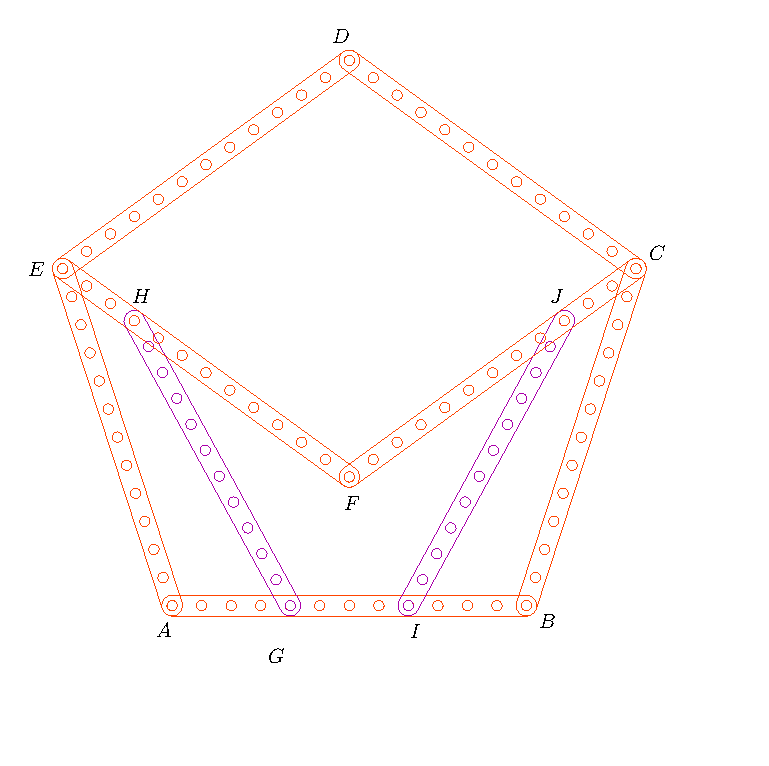
\includegraphics[scale=1]{12/penta12b}
 \caption{Pentagon size 12 case (b).}
 \label{fig:penta12b}
\end{figure}

Figure \ref{fig:penta12b} show a regular pentagon $A,B,C,D,E$ of size 12 with a rhombus $D,I,H,G$ of size $12$. We prove strips $GH,IJ$ are correct. First we calculate the abscissas going through vertices $G,A,E,H$ substracting when we move to the left and adding when we move to the right:
\begin{align}
GH_x &= -GA_x - AE_x + EH_x\\
 &= -\overline{GA} - \overline{AE}\cos\left(\frac{2\pi}5\right)
 +\overline{EH}\cos\left(\frac{\pi}5\right)\nonumber\\
 &= -4 - 12\left(\frac{\sqrt5 - 1}4\right) + 3\left(\frac{1+\sqrt5}4\right)
 = \frac{-1-9\sqrt5}4
\end{align}

Then we calculate the ordinates going to the same order of vertices adding when we go up and substracting when we go down:
\begin{align}
GH_y &= AG_y + AE_y - EH_y\\
 &= 0 + \overline{AE}\sin\left(\frac{2\pi}5\right)
 - \overline{EH}\sin\left(\frac{\pi}5\right)\nonumber\\
 &= 12\left(\frac{\sqrt{10+2\sqrt5}}4\right)
 - 3\left(\frac{\sqrt{10-2\sqrt5}}4\right)\nonumber\\
 &= \frac{12\sqrt{10+2\sqrt5} -3\sqrt{10-2\sqrt5}}4 = \frac{\sqrt{1530-18\sqrt5}}4
\end{align}

Finally we calculate the distance $\overline{GH}$ which coincides with strip size $11$:
\begin{align}
\overline{GH} &= \sqrt{(GH_x)^2 + (GH_y)^2}\\
 &= \sqrt{\left(\frac{-1-9\sqrt5}{4}\right)^2 + \frac{1530-18\sqrt5}{16}}\nonumber\\
 &= \sqrt{\frac{406+18\sqrt5}{16} + \frac{1530-18\sqrt5}{16}} = \sqrt{121} = 11
\end{align}


\section{Pentagon of size 11}

\begin{figure}[h]
 \centering
 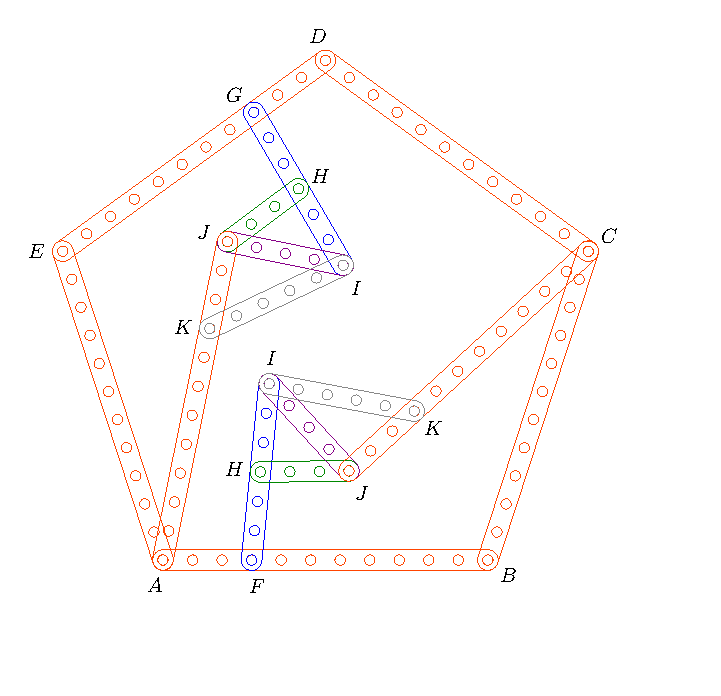
\includegraphics[scale=1]{11/penta11a}
 \caption{Pentagon size 11.}
 \label{fig:penta11a}
\end{figure}

Figure \ref{fig:penta11a} show a rigid regular pentagon $A,B,C,D,E$ of size 11. A program found this is the smallest pentagon having a consecutive sides diagonal of the form $\dfrac{z_2 + z_3\sqrt5}{z_1}$ instead of the nested form $\dfrac{z_2\sqrt{z_3+z_4\sqrt5}}{z_1}$ where $z_i$ are integers. The mentioned diagonal is the distance $\overline{CF}$ in the figure which can be calculated with the law of cosines knowing angle $\angle{CBF} = \dfrac{3\pi}5$ and denesting the result. We calculate the angle $\angle{CFB}$ for the drawing:
\begin{align}
\overline{CF}^2 &= \overline{BC}^2 + \overline{BF}^2 
 - 2(\overline{BC})(\overline{BF})\cos\left(\dfrac{3\pi}5\right)\\
 &= 11^2 + 8^2 - 2(11)(8)\left(\frac{1-\sqrt5}4\right) = 141 + 44\sqrt5\nonumber\\
\overline{CF} &= \sqrt{141 + 44\sqrt5} = 11 + 2\sqrt5\\
\cos(\angle{CFB}) &= \frac{\overline{CF}^2 + \overline{BF}^2 - \overline{BC}^2}
 {2(\overline{CF})(\overline{BF})}\nonumber\\
 &= \frac{141+44\sqrt5 + 8^2 - 11^2}{2(11+2\sqrt5)(8)}
  = \frac{21+11\sqrt5}{44+8\sqrt5} = \frac{121+79\sqrt5}{404}
\end{align}

\subsection{Five strips build distance $11+2\sqrt{5}$}

A five strips cluster can create a rigid distance like $11 + 2\sqrt{5}$. In the figure, three strips $\overline{FI} = 2\overline{HJ}, \overline{FI} > \overline{IJ}$ builds a right angle $\angle{FJI} = \pi$, since triangle $\triangle{IJH}$ is isosceles ($\overline{FH} = \overline{HI} = \overline{JH}$). These three strips also build a distance $\overline{FJ} = \sqrt{\overline{FI}^2 - \overline{IJ}^2} = \sqrt{6^2 - 4^2} = 2\sqrt5$. Now we attach strip $\overline{CJ}$ making a second right triangle $\angle{CJI} = \pi$ using strip $\overline{IK}=5$ as pythagorean diagonal ($\overline{JK}=3, \overline{IJ}=4$). We have two right triangles at vertice $J$ so vertices $F,J,C$ are collinear, so we can calculate the distance $\overline{FC} = \overline{CJ} + \overline{JF} = 11 + 2\sqrt5$. We repeat the five-strips cluster between vertices $A,G$ preventing overlaps of any strips. Since the clusters are rigid we formed two rigid triangles $\triangle{ABC}, \triangle{DEA}$ so the pentagon is rigid.
\\\\
The program found the next pentagon of this type is a lot bigger: $\overline{BC}=246, \overline{BF}=70, \overline{CF}=41+105\sqrt5$.

\section{Pentagon of size 10}

\begin{figure}[h]
 \centering
 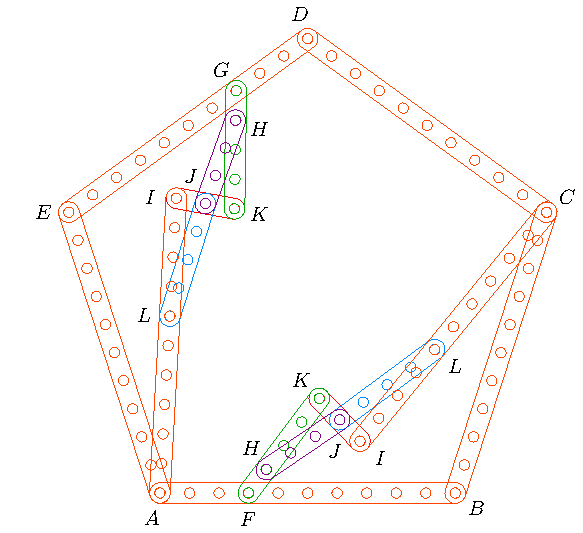
\includegraphics[scale=1]{10/penta10a}
 \caption{Pentagon size 10.}
 \label{fig:penta10a}
\end{figure}

Figure \ref{fig:penta10a} show a rigid regular pentagon $A,B,C,D,E$ of size 10. We calculate a diagonal joining to consecutive sides relative primes to have something exclusive to the size 10, we choose $\overline{BF}:\overline{BC} = 7:10$. With the law of cosines we calculate $\overline{CF}$.
We calculate the angle $\angle{CFB}$ for the drawing:
\begin{align}
\overline{CF}^2 &= \overline{BC}^2 + \overline{BF}^2
 - 2(\overline{BC})(\overline{BF})\cos\left(\frac{3\pi}5\right)\nonumber\\
 &= 10^2 + 7^2 - 2(10)(7)\left(\frac{1-\sqrt5}4\right) = 114 + 35\sqrt5\\
\overline{CF} &= \sqrt{114 + 35\sqrt5} \\
\cos(\angle{CFB}) &= \frac{\overline{CF}^2 + \overline{BF}^2 - \overline{BC}^2}
 {2(\overline{CF})(\overline{BF})}\nonumber\\
 &= \frac{114+35\sqrt5 + 7^2 - 10^2}{2(\sqrt{114 + 35\sqrt5})(7)}
  = \frac{9+5\sqrt5}{2\sqrt{114+35\sqrt5}}
\end{align}

\subsection{Five strips for distance $\sqrt{114+35\sqrt5}$}

\begin{figure}[h]
 \centering
 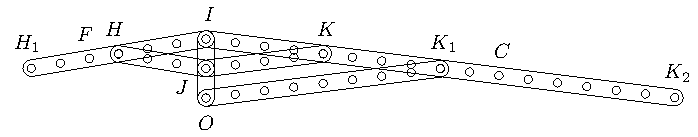
\includegraphics[scale=1.3]{11/cluster11a}
 \caption{Five strips cluster for distance $\overline{CF} = \sqrt{114+35\sqrt5}$}
 \label{fig:cluster11a}
\end{figure}

Number $\sqrt{114 + 35\sqrt5}$ cannot be denested so we need to solve this with a cluster of strips. A program found a lot of solutions for this distance using five strips, so we choose one narrow enough to fit inside the decagon.
\\\\
Figure \ref{fig:cluster11a} shows how to prove the cluster distance is correct. In the figure we have two isoscelles triangles $\triangle{IJH}$ and $\triangle{IOK_1}$. The sides $IH$ and $IK_1$ are extended to double the original size so we have two vertices $H_1$ and $K_2$ so we have to right angles $\angle{IJH_1}$ and $\angle{IOK_2}$.
\\\\
According to the figure $\overline{OM_1}=1$ and $\overline{OM_2}=6$ so $\overline{M_1M_2} = \sqrt{(\overline{OM_2})^2 + (\overline{OM_1})^2} = \sqrt{6^2-1^2} = \sqrt{35}$.

Also  $\overline{ON_1}=2$ and $\overline{N_1N_2}=16$ so $\overline{ON_2} = \sqrt{(\overline{N_1N_2})^2 - (\overline{ON_1})^2} = \sqrt{16^2 - 2^2} = 6\sqrt{7}$.

Then we calculate the abscissas $M_x,N_x$ and ordinates $M_y,N_y$ of vertices $M,N$ noting $M$ is located at fraction $\frac{4}{6}$ of distance of vertices $O,M_2$ and $N$ is located at fraction $\frac{10}{16}$ of distance of vertices $N1,N2$. Assuming vertice $O$ is located at the origin we have:
\begin{align}
M_x &= \frac{4}{6}\overline{OM_1} = \frac{2}{3}(1) = \frac{2}3\\
M_y &= \frac{4}{6}\overline{M_1M_2} = \frac{2}{3}\sqrt{35}\\
N_x &= \overline{ON_1} - \frac{10}{16}\overline{ON_1} = 2 - \frac{5}{8}(2) = \frac{3}4\\
N_y &= -\frac{10}{16}\overline{ON_2} = -\frac{5}{8}\left(6\sqrt7\right) = -\frac{15}{4}\sqrt{7}
\end{align}
Finally we calculate the distance $\overline{MN}$:
\begin{align}
\overline{MN} &= \sqrt{(M_x - N_x)^2 + (M_y - N_y)^2}\\
 &= \sqrt{\left(\dfrac{2}3 - \dfrac{3}4\right)^2 
 + \left(\dfrac{2}{3}\sqrt{35} + \dfrac{15}{4}\sqrt{7}\right)^2}\nonumber\\
 &= \sqrt{\dfrac{1}{144} + \dfrac{140}9 + 35\sqrt5 + \dfrac{1575}{16}} = \sqrt{114+35\sqrt5}
\end{align}

\end{document}